% !TeX root = ../CCNUthesis-doc.tex

\section{使用说明}

\subsection{基本用法}

以下是一份简单的 \TeX{} 文档,它演示了 \cls{CCNUthesis} 的最基本用法:

\begin{latexexample}[deletetexcs={\documentclass},
    moretexcs={\chapter},morekeywords={\documentclass},
    emph={[2]document}]
  % main.tex
  \documentclass{CCNUthesis}
  \begin{document}
    \chapter{欢迎}
    \section{Welcome to CCNUthesis!}
    你好,\LaTeX{}!
  \end{document}
\end{latexexample}


按照~\ref{subsec:编译方式} 小节中的方式编译该文档,您应当得到一篇 3 页的文章。

% 英文模板可以用类似的方式使用:

% \begin{latexexample}[deletetexcs={\documentclass},
%     moretexcs={\chapter},morekeywords={\documentclass},
%     emph={[2]document}]
%   % thesis-en.tex
%   \documentclass{CCNUthesis-en}
%   \begin{document}
%     \chapter{Welcome}
%     \section{Welcome to CCNUthesis!}
%     Hello, \LaTeX{}!
%   \end{document}
% \end{latexexample}

% 英文模板只对正文部分进行了改动,封面、指导小组成员以及声明页仍将
% 显示为中文。

\subsection{编译方式} \label{subsec:编译方式}

本模板不支持 \pdfTeX{} 引擎,仅支持使用 \XeLaTeX{} 。为了生成正确的目录、脚注以及交叉引用,您至少需要连续编译两次。

以下代码中,假设您的 \TeX{} 源文件名为 \file{main.tex}。请在命令行中执行
\begin{shellexample}[morekeywords={xelatex}]
  xelatex main
\end{shellexample}

如果您想要编译参考文献,在 \file{CCNUthesis-main.bib} 中输入正确的条目信息并在正文中正确引用之后(引用方式见~\ref{para:参考文献引用}),请使用“\pkg{biber}”编译链,即在命令行中一次执行下面四条命令:
\begin{shellexample}[morekeywords={biber}]
  xelatex main
  biber main
  xelatex main
  xelatex main
\end{shellexample}
或使用 \pkg{latexmk}:
\begin{shellexample}[morekeywords={latexmk}]
  latexmk main
\end{shellexample}


\subsection{模板选项} \label{subsec:模板选项}

所谓“模板选项”,指需要在引入文档类的时候指定的选项:
\begin{latexexample}[deletetexcs={\documentclass},
    morekeywords={\documentclass}]
  \documentclass(*\oarg{模板选项}*){CCNUthesis}
\end{latexexample}

有些模板选项为布尔型,它们只能在 \opt{true} 和 \opt{false}
中取值。对于这些选项,\kvopt{\meta{选项}}{true} 中的“|= true|”
可以省略。

下面用形如“【本|硕|博】”表示该命令或环境的适用范围,比如“【硕|博】”表示输入之后仅对硕博模板起作用,对本科模板不起作用(作用范围的设置往往来源于格式规范的要求等),其余“【本】”等同理解释。


\begin{function}{type}
  \begin{ccnusyntax}[emph={[1]type}]
    type = (*<doctor|master|(bachelor)>*)
  \end{ccnusyntax}
  选择论文类型。三种选项分别代表博士学位论文、硕士学位论文和本科
  毕业论文。
\end{function}

\begin{function}[updated = 2024-03-19]{version}
  \begin{ccnusyntax}[emph={[1]version}]
    version = (*<(electronic)|print-master-oneside|print-master-twoside|print-doctor>*)
  \end{ccnusyntax}
  文档版本。
\end{function}

\begin{itemize}
  \item electronic:电子版,无空白页(本科选择这个即可,单双打印皆可,答辩时可以双面打印,纸质版终稿教务处要求单面打印)
  \item print-master-oneside:打印版,硕士,无空白页,单面打印,封面的 logo 和页眉的 logo 变成黑色
  \item print-master-twoside:打印版,硕士,有空白页,双面打印,封面的 logo 和页眉的 logo 变成黑色
  \item print-doctor:打印版,博士,有空白页,双面打印,封面的 logo 和页眉的 logo 变成黑色
\end{itemize}

注意:对于硕博的模板,\parencite{研究生院研究生学位论文规范} 中提到的“封面、原创性声明和使用授权书采用单面印刷,中英文扉页、摘要及后续内容采用双面印刷(硕士学位论文可以单面印刷)。” 实现方式即为在所需要单面印刷的后面加一页空白页,然后全部双面打印即可,这个就是上面键值的设计想法,用户不需要自己手动加空白页,只需要选择自己对应所需版本就会对应自动判断是否添加空白页。


\begin{function}[added = 2023-04-07,updated = 2024-04-03]{blind-version}
  \begin{ccnusyntax}[emph={[1]blind-version}]
    blind-version = (*<true|false|remove-partial-schoolname|remove-all-schoolname|blind-schoolname>*)
  \end{ccnusyntax}
  【本|硕|博】盲审版本。
  \begin{itemize}
    \item 【本|硕|博】\kvopt{blind-version}{true} 或省略 \opt{true} (即只写 \opt{blind-version}) 都表示开启盲审版本,校名、姓名、导师姓名、职称、版权声明页会去掉,并且去掉页眉。
    \item 【本|硕|博】\kvopt{blind-version}{false} 或者不写 \opt{blind-version} 键值表示不开启。
    \item 【本】\kvopt{blind-version}{remove-partial-schoolname}:去掉封面和版权声明页第一行中“华中师范”四个字(此键值只是为了实现邓国泰老师在旧模板中的做法)
    \item 【本】\kvopt{blind-version}{remove-all-schoolname}:去掉封面的“华中师范大学”校名以及版权声明页第一行中“华中师范大学”但保留版权声明页
    \item 【硕|博】\kvopt{blind-version}{blind-schoolname}:去掉封面的“华中师范大学”校名,版权声明页第一行中“华中师范大学”变成“XXXXXX”
  \end{itemize}
  \emph{注意致谢、参考文献等的盲审处理需要用户自行处理,本模板提供了 \tn{blind} 命令(见 \ref{subsubsec:豹尾}节)来处理致谢中的人名,不过一切以学院的要求为准。}
\end{function}


\begin{function}[added = 2024-04-03]{copyright-version}
  \begin{ccnusyntax}[emph={[1]copyright-version}]
    copyright-version = (*<(old)|new>*)
  \end{ccnusyntax}
  【硕|博】版权页版本。
  \begin{itemize}
    \item \kvopt{copyright-version}{old} 表示使用旧版权页。对应 \file{copyright/Originality_Copyright_master_doctor_old.pdf}
    \item \kvopt{copyright-version}{new} 表示使用新版权页。对应 \file{copyright/Originality_Copyright_master_doctor_new.pdf}
  \end{itemize}
\end{function}

% \begin{function}{oneside,twoside}
%   指明论文的单双面模式,默认为 \opt{twoside}。该选项会影响每章
%   的开始位置,还会影响页眉样式。
% \end{function}

% 在双面模式(\opt{twoside})下,按照通常的排版惯例,每章应只从
% 奇数页(在右)开始;而在单页模式(\opt{oneside})下,则可以从
% 任意页面开始。本模板中,目录、摘要、符号表等均视作章,也按相同
% 方式排版。

% 双面模式下,正文部分偶数页(在左)的左页眉显示章标题,奇数页
% (在右)的右页眉显示节标题;前置部分的页眉按同样格式显示,但文字
% 均为对应标题(如“目录”、“摘要”等)。
% 而在单面模式下,正文部分则页面不分奇偶,均同时显示左、右页眉,
% 文字分别为章标题和节标题;前置部分只有中间页眉,显示对应标题。

\begin{function}{draft}
  \begin{ccnusyntax}[emph={[1]draft}]
    draft = (*<\TFF>*)
  \end{ccnusyntax}
  【本|硕|博】选择是否开启草稿模式,默认关闭。
\end{function}

草稿模式为全局选项,会影响到很多宏包的工作方式。
开启之后,主要的变化有:
\begin{itemize}
  \item 把行溢出的盒子显示为黑色方块;
  \item 不实际插入图片,只输出一个占位方框;
  \item 关闭超链接渲染,也不再生成 PDF 书签;
  \item 显示页面边框。
\end{itemize}

% \begin{function}[added=2018-01-31]{config}
%   \begin{ccnusyntax}[emph={[1]config}]
%     config = (*\marg{文件}*)
%   \end{ccnusyntax}
%   用户配置文件的文件名。默认为空,即不载入用户配置文件。
% \end{function}


\subsection{参数设置}

\begin{function}{\ccnusetup}
  \begin{ccnusyntax}[morekeywords={\ccnusetup}]
    \ccnusetup(*\marg{键值列表}*)
  \end{ccnusyntax}
  【本|硕|博】本模板提供了一系列选项,可由您自行配置。载入文档类之后,以下
  所有选项均可通过统一的命令 \cs{ccnusetup} 来设置。
\end{function}

\cs{ccnusetup} 的参数是一组由(英文)逗号隔开的选项列表,列表中的
选项通常是 \kvopt{\meta{key}}{\meta{value}} 的形式。部分选项的
\meta{value} 可以省略。对于同一项,后面的设置将会覆盖前面的设置。
在下文的说明中,将用\textbf{粗体}表示默认值。

\cs{ccnusetup} 采用 \LaTeX3 风格的键值设置,支持不同类型以及多种
层次的选项设定。键值列表中,“|=|”左右的空格不影响设置;但需注意,
参数列表中\emph{不可以出现空行}。

与模板选项相同,布尔型的参数可以省略 \kvopt{\meta{选项}}{true}
中的“\kvopt{}{true}”。

另有一些选项包含子选项,如 \opt{style} 和 \opt{info} 等。它们可以
按如下两种等价方式来设定:

\begin{latexexample}[morekeywords={\ccnusetup},
    emph={[1]style,cjk-font,info,title,title*,author,author*,department}]
  \ccnusetup{
    style = {cjk-font = mac},
    info  = {
      title      = {论动体的电动力学},
      title*     = {On the Electrodynamics of Moving Bodies},
      author     = {阿尔伯特·爱因斯坦},
      author*    = {Albert Einstein},
      department = {物理学系}
    }
  }
\end{latexexample}

或者

\begin{latexexample}[morekeywords={\ccnusetup},
    emph={[1]style,cjk-font,info,title,title*,author,author*,department}]
  \ccnusetup{
    style/cjk-font  = mac,
    info/title      = {论动体的电动力学},
    info/title*     = {On the Electrodynamics of Moving Bodies},
    info/author     = {阿尔伯特·爱因斯坦},
    info/author*    = {Albert Einstein},
    info/department = {物理学系}
  }
\end{latexexample}


注意 “|/|” 的前后均不可以出现空白字符。


\subsubsection{论文格式} \label{subsubsec:论文格式}

\begin{function}{style}
  \begin{ccnusyntax}[emph={[1]style}]
    style = (*\marg{键值列表}*)
    style/(*\meta{key}*) = (*\meta{value}*)
  \end{ccnusyntax}
  【本|硕|博】该选项包含许多子项目,用于设置论文格式。具体内容见下。
\end{function}


\begin{function}{style/font}
  \begin{ccnusyntax}[emph={[1]font}]
    font = (*<newtx|(times)|stixtwo|xits|tg|none>*)
  \end{ccnusyntax}
  【本|硕|博】设置西文字体(包括数学字体)。具体配置见表~\ref{tab:font}。
\end{function}

% \begin{table}[ht]
% \centering
% \begin{threeparttable}
%   \caption{西文字体配置}
%   \label{tab:font}
%   \small
%   \begin{tabular}{ccccc}
%     \toprule
%       & \textbf{正文字体} & \textbf{无衬线字体} & \textbf{等宽字体} & \textbf{数学字体} \\
%     \midrule
%       |garamond|        & EB Garamond         & Libertinus Sans & LM Mono\tnote{a} & Garamond Math   \\
%       |libertinus|      & Libertinus Serif    & Libertinus Sans & LM Mono          & Libertinus Math \\
%       |lm|              & LM Roman            & LM Sans         & LM Mono          & LM Math         \\
%       |palatino|        & TG Pagella\tnote{b} & Libertinus Sans & LM Mono          & TG Pagella Math \\
%       |times|           & XITS                & TG Heros        & TG Cursor        & XITS Math       \\
%       |times*|\tnote{c} & Times New Roman     & Arial           & Courier New      & XITS Math       \\
%     \bottomrule
%   \end{tabular}
%   \begin{tablenotes}
%     \item[a] “LM”是 Latin Modern 的缩写。
%     \item[b] “TG”是 TeX Gyre 的缩写。
%     \item[c] 本行中,Times New Roman、Arial 和 Courier New 是商业字体,
%       不包含在 \TeXLive{} 发行版中,但在 Windows 和 macOS 系统上均默认安装。
%   \end{tablenotes}
% \end{threeparttable}
% \end{table}
\begin{table}[htbp]
  \centering
  \begin{threeparttable}
    \caption{西文字体配置}
    \label{tab:font}
    \small
    \begin{tabular}{ccccc}
      \toprule
        & \textbf{正文字体} & \textbf{无衬线字体} & \textbf{等宽字体} & \textbf{数学字体} \\
      \midrule
      |stixtwo| & STIX Two Text   & TG Heros\tnote{a} & TG Cursor   & STIX Two Math \\
      |xits |   & XITS            & TG Heros & TG Cursor   & XITS Math \\
      |times|\tnote{b}   & Times New Roman & Arial    & Courier New & newtxmath \\
      |newtx|   & TG Termes   & TG Heros & TG Cursor   & newtxmath \\
      |tg|      & TG Termes       & TG Heros & TG Cursor   & TG Termes Math \\
      \bottomrule
    \end{tabular}
    \begin{tablenotes}
      % \item[a] “LM”是 Latin Modern 的缩写。
      \item[a] “TG”是 TeX Gyre 的缩写。
      \item[b] 本行中,Times New Roman、Arial 和 Courier New 是商业字体,
        不包含在 \TeXLive{} 发行版中,但在 Windows 和 macOS 系统上均默认安装。
    \end{tablenotes}
  \end{threeparttable}
  \end{table}


\begin{function}{style/cjk-font}
  \begin{ccnusyntax}[emph={[1]cjk-font}]
    cjk-font = (*<adobe|(fandol)|founder|mac|sinotype|sourcehan|windows|none>*)
  \end{ccnusyntax}
  【本|硕|博】设置中文字体。具体配置见表~\ref{tab:cjk-font}。
\end{function}

\begin{table}[htbp]
  \caption{中文字体配置}
  \label{tab:cjk-font}
  \centering
  \small
  \begin{tabular}{ccccc}
    \toprule
      & \textbf{正文字体(宋体)} & \textbf{无衬线字体(黑体)} & \textbf{等宽字体(仿宋)} & \textbf{楷体} \\
    \midrule
      |adobe|     & Adobe 宋体      & Adobe  黑体     & Adobe  仿宋  & Adobe 楷体      \\
      |fandol|    & Fandol 宋体     & Fandol 黑体     & Fandol 仿宋  & Fandol 楷体     \\
      |founder|   & 方正书宋        & 方正黑体        & 方正仿宋     & 方正楷体        \\
      |mac|       & (华文)宋体-简 & (华文)黑体-简 & 华文仿宋     & (华文)楷体-简 \\
      |sinotype|  & 华文宋体        & 华文黑体        & 华文仿宋     & 华文楷体        \\
      |sourcehan| & 思源宋体        & 思源黑体        & ---          & ---             \\
      |windows|   & (中易)宋体    & (中易)黑体    & (中易)仿宋 & (中易)楷体    \\
    \bottomrule
  \end{tabular}
\end{table}

启用 \kvopt{font}{none} 或 \kvopt{cjk-font}{none} 之后,模板将关闭
默认西文 / 中文字体设置。此时,您需要自行使用 \cs{setmainfont}、
\cs{setCJKmainfont}、\cs{setmathfont} 等命令来配置字体。


% \begin{function}{style/font-size}
%   \begin{ccnusyntax}[emph={[1]font-size}]
%     font-size = (*<(-4)|5>*)
%   \end{ccnusyntax}

%   设置论文的基础字号。
% \end{function}


\begin{function}{style/fullwidth-stop}
  \begin{ccnusyntax}[emph={[1]fullwidth-stop}]
    fullwidth-stop = (*<catcode|mapping|(false)>*)
  \end{ccnusyntax}
  【本|硕|博】选择是否把全角实心句点\FSFW 作为默认的句号形状。
  这种句号一般用于科技类文章,以避免与下标“$_o$”或“$_0$”混淆。
\end{function}

选择 \kvopt{fullwidth-stop}{catcode} 或 \opt{mapping} 后,都会实现上述效果。
有所不同的是,在选择 \opt{catcode} 后,只有\emph{显式的}\FSID 会被替换
为\FSFW;但在选择 \opt{mapping} 后,\emph{所有的}\FSID 都会被替换。例如,
如果您用宏保存了一些含有\FSID 的文字,那么在选择 \opt{catcode} 时,其中
的\FSID 不会将被替换为\FSFW。

选项 \kvopt{fullwidth-stop}{mapping} 只在 \XeTeX{} 下有效。

如果您在选择 \kvopt{fullwidth-stop}{mapping} 后仍需要临时显示\FSID,
可以按如下方法操作:
\begin{latexexample}[moretexcs={\CJKfontspec},emph={[1]Mapping}]
  % 请使用 XeTeX 编译
  % 外侧的花括号表示分组
  这是一个句号{\CJKfontspec{(*\meta{字体名}*)}[Mapping=full-stop]。}
\end{latexexample}

\begin{function}{style/footnote-style}
% 这里奇怪的东西是用来控制对齐的。ccnusyntax 会吃掉开头的几个空格,因此这里用 X 来占位。
  \begin{ccnusyntax}[emph={[1]footnote-style}]
    footnote-style = (*<plain|\\
      XXXX\mbox{}~~~~~~~~~~~~~~~~~libertinus|libertinus*|libertinus-sans|\\
      XXXX\mbox{}~~~~~~~~~~~~~~~~~pifont|pifont*|pifont-sans|pifont-sans*|\\
      XXXX\mbox{}~~~~~~~~~~~~~~~~~xits|xits-sans|xits-sans*>*)
  \end{ccnusyntax}
  【本|硕|博】设置脚注编号样式。西文字体设置会影响其默认取值(见
  表~\ref{tab:footnote-font})。因此,要使得该选项生效,需将其
  放置在 \opt{font} 选项之后。带有 |sans| 的为相应的无衬线字体
  版本;带有 |*| 的为阴文样式(即黑底白字)。
\end{function}

\begin{table}[ht]
  \caption{西文字体与脚注编号样式默认值的对应关系}
  \label{tab:footnote-font}
  \centering
  \small
  \begin{tabular}{ccccc}
    \toprule
      \textbf{西文字体设置} &
        |libertinus| & |lm|     & |palatino| & |times| \\
    \midrule
      \textbf{脚注编号样式默认值} &
        |libertinus| & |pifont| & |pifont|   & |xits|  \\
    \bottomrule
  \end{tabular}
\end{table}

\begin{function}{style/caption-labelstyle}
  \begin{ccnusyntax}[emph={[1]caption-labelstyle}]
    caption-labelstyle = (*<arabic|(hyphen)|dot>*)
  \end{ccnusyntax}
  【本|硕|博】图表标题 label 计数样式。

  \begin{itemize}
    \item \opt{arabic}:图1,图2... 跨 chapter 连续编号,即若上一个 chapter 的图编号为 4,下一个 chapter 的第一个图编号为5
    \item \opt{hyphen}:图1-1,图1-2,图2-1...其中图 $x$-$y$,$x$ 表示 chapter 的值,$y$ 表示该 chapter 的计数器值(通俗理解就是此 chapter 的第 $y$ 张图或表),$y$ 在新的 chapter 会自动重新开始计数
    \item \opt{dot}:图1.1,图1.2,图2.1...其中图 $x$.$y$,$x,y$ 的含义同上
  \end{itemize}
\end{function}

\begin{function}{style/caption-labelseperator}
  \begin{ccnusyntax}[emph={[1]caption-labelseperator}]
    caption-labelseperator = (*<(colon)|space>*)
  \end{ccnusyntax}
  【本|硕|博】图表标题 label 和标题内容之间的分隔符

  \begin{itemize}
    \item \opt{colon}:表示 「:␣」,即一个西文冒号加一个空格
    \item \opt{space}:表示 「␣␣」,即两个空格
  \end{itemize}
\end{function}

\begin{function}[added = 2022-06-04]{style/chapter-breakstyle}
  \begin{ccnusyntax}[emph={[1]chapter-breakstyle}]
    caption-labelseperator = (*<(continuous)|newpage>*)
  \end{ccnusyntax}
  【本】控制 \tn{chapter} 是否新起一页。根据 \parencite{研究生院研究生学位论文规范},硕博模板的 \tn{chapter} 是新起一页的,故此键值设计仅对本科模板生效。

  \begin{itemize}
    \item \opt{continuous}:不新起一页,接着上一个 \tn{chapter} 连续排版
    \item \opt{newpage}:\tn{chapter} 会新起一页开始排版
  \end{itemize}
\end{function}

\begin{function}[added = 2022-06-20]{style/show-head}
  \begin{ccnusyntax}[emph={[1]show-head}]
    show-head = (*<\TTF>*)
  \end{ccnusyntax}
  【硕|博】是否显示页眉。统一控制页眉 logo 和页眉线的显示与否。
\end{function}


\begin{function}[updated = 2022-06-20]{style/show-headlogo}
  \begin{ccnusyntax}[emph={[1]show-headlogo}]
    show-headlogo = (*<\TFF>*)
  \end{ccnusyntax}
  【硕|博】是否显示页眉 logo。具体 logo 样式见图~\ref{figure:headlogo}。
\end{function}

\begin{figure}[htbp]
  \centering
  \begin{minipage}{0.45\textwidth}
    
\includegraphics[height = 2cm]{masterlogo.png}
  \end{minipage}
  \begin{minipage}{0.45\textwidth}
    
\includegraphics[height = 2cm]{doctorlogo.png}
  \end{minipage}
  \caption{headlogo}
  \label{figure:headlogo}
\end{figure}

\begin{function}{style/headline}
  \begin{ccnusyntax}[emph={[1]headline}]
    headline = (*<single|double|thin-thick|thick-thin|(none)>*)
  \end{ccnusyntax}
  【硕|博】页眉线的样式。

  \begin{itemize}
    \item \opt{single}:一条线
    \item \opt{double}:两条线,一样粗细
    \item \opt{thin-thick}:两条线,上细下粗(文武线)
    \item \opt{thick-thin}:两条线,上粗下细(武文线)
    \item \opt{none}:页眉没有线
  \end{itemize}
\end{function}

\begin{function}[added = 2022-6-19]{style/head-scope}
  \begin{ccnusyntax}[emph={[1]head-scope}]
    head-scope = (*<all|(main)>*)
  \end{ccnusyntax}
  【硕|博】页眉线的作用范围。

  \begin{itemize}
    \item \opt{all}:除了全文的第一页封面,其他页面均有页眉。
    \item \opt{main}:正文开始才有页眉。
  \end{itemize}
\end{function}

\begin{function}[added = 2022-06-18]{style/keywords-newline}
  \begin{ccnusyntax}[emph={[1]keywords-newline}]
    keywords-newline = (*\TTF*)(硕|博)
    keywords-newline = (*\TFF*)(本)
  \end{ccnusyntax}
  【本|硕|博】(中英统一控制)摘要和关键词之间是否空一行。

  \begin{itemize}
    \item \opt{true}:摘要和关键词之间空一行
    \item \opt{false}:摘要新起一段后为关键词
  \end{itemize}
\end{function}

\begin{function}[added = 2022-06-19]{style/listoffigures-show,style/listoftables-show}
  \begin{ccnusyntax}[emph={[1]listoffigures-show,listoftables-show}]
    listoffigures-show = (*\TTF*)(硕|博)
    listoftables-show = (*\TTF*)(硕|博)
    listoffigures-show = (*\TFF*)(本)
    listoftables-show = (*\TFF*)(本)
  \end{ccnusyntax}
  【本|硕|博】控制是否显示图表目录。若都显示则紧跟文章目录后,且图目录在表目录前。
\end{function}

\begin{function}[added = 2022-06-19]{style/listoffigures-name,style/listoftables-name}
  \begin{ccnusyntax}[emph={[1]listoffigures-name,listoftables-name}]
    listoffigures-name = (*<\marg{图目录的节标题}>*)
    listoftables-name = (*<\marg{表目录的节标题}>*)
  \end{ccnusyntax}
  【本|硕|博】图表目录的节标题。分别默认为 |插 \quad 图| 和 |表 \quad 格|
\end{function}


\begin{function}{style/hyperlink}
  \begin{ccnusyntax}[emph={[1]hyperlink}]
    hyperlink = (*<color|(none)>*)
  \end{ccnusyntax}
  【本|硕|博】设置超链接样式。\opt{color} 表示用彩色显示超链接;\opt{none} 表示没有特殊装饰,可用于生成最终的打印版文稿。
\end{function}

\begin{function}{style/hyperlink-color}
  \begin{ccnusyntax}[emph={[1]hyperlink-color}]
    hyperlink-color = (*<(default)|classic|material|graylevel|prl>*)
  \end{ccnusyntax}
  【本|硕|博】设置超链接颜色。该选项在 \kvopt{hyperlink}{none} 时无效。
  各选项所代表的颜色见表~\ref{tab:hyperlink-color}。
\end{function}


\begin{table}[ht]
\centering
\small

\newcommand\linkcolorexam[3]{%
  {\small 图~\textcolor[HTML]{#1}{1-2},
    (\textcolor[HTML]{#1}{3.4})~式} &
  {\small \textcolor[HTML]{#2}{\texttt{https://g.cn}}} &
  {\small 文献~[\textcolor[HTML]{#3}{1}],
    (\textcolor[HTML]{#3}{Knuth~1986})}}
\begin{threeparttable}
\caption{预定义的超链接颜色方案}
\label{tab:hyperlink-color}
\begin{tabular}{c*{3}{>{\hspace{0.2cm}}c<{\hspace{0.2cm}}}}
  \toprule
    \textbf{选项} & \textbf{链接} & \textbf{URL} & \textbf{引用} \\

  \midrule
    \opt{default}            & \linkcolorexam{990000}{0000B2}{007F00} \\
    \opt{classic}            & \linkcolorexam{FF0000}{0000FF}{00FF00} \\
    \opt{material}\tnote{a}  & \linkcolorexam{E91E63}{009688}{4CAF50} \\
    \opt{graylevel}\tnote{a} & \linkcolorexam{616161}{616161}{616161} \\
    \opt{prl}\tnote{b}       & \linkcolorexam{2D3092}{2D3092}{2D3092} \\
  \bottomrule
\end{tabular}
\begin{tablenotes}

  \item[a] 取自 Material 色彩方案
    (见 \url{https://material.io/guidelines/style/color.html})。
  \item[b] \textit{Physical Review Letter} 杂志配色。

\end{tablenotes}
\end{threeparttable}
\end{table}



% \begin{function}{style/bib-backend}
%   \begin{ccnusyntax}[emph={[1]bib-backend}]
%     bib-backend = (*<bibtex|biblatex>*)
%   \end{ccnusyntax}

%   选择参考文献的支持方式。选择 \opt{bibtex} 后,将使用 \BibTeX{}
%   处理文献,样式由 \pkg{natbib} 宏包负责;选择 \opt{biblatex} 后,
%   将使用 \biber{} 处理文献,样式则由 \pkg{biblatex} 宏包负责。
% \end{function}

\begin{function}[updated = 2023-03-11]{style/bib-style}
  \begin{ccnusyntax}[emph={[1]bib-style}]
    bib-style = (*<(ccnu-bachelor-numerical)|ccnu-bachelor-author-year|ccnu-master|ccnu-doctor|gb7714-2015|gb7714-2015ay>*)
  \end{ccnusyntax}
  【本|硕|博】设置参考文献样式。
  \begin{itemize}
    \item \opt{ccnu-bachelor-numerical}:参考 \parencite{本科生院毕业论文注释与参考文献著录格式} 定制的参考文献格式,顺序编码制
    \item \opt{ccnu-bachelor-author-year}:和 \opt{ccnu-bachelor-numerical} 格式相同,著者—出版年制
    \item \opt{ccnu-master}:国家标准 GB/T 7714--2015 的顺序编码制
    \item \opt{ccnu-doctor}:国家标准 GB/T 7714--2015 的顺序编码制
    \item \opt{gb7714-2015}:国家标准 GB/T 7714--2015 的顺序编码制
    \item \opt{gb7714-2015ay}:国家标准 GB/T 7714--2015 的作者-年制
  \end{itemize}
  % \opt{author-year} 和 \opt{numerical} 分别对应国家标准 GB/T 7714--2015 \cite{gb-t-7714-2015} 中的著者—出版年制和顺序编码制。
  % 选择 \meta{其他样式} 时,如果 \kvopt{bib-backend}{bibtex},需保证相应的 \file{.bst} 格式文件能被调用;而如果\kvopt{bib-backend}{biblatex},则需保证相应的 \file{.bbx} 格式文件能被调用。
\end{function}

% \begin{function}{style/cite-style}
%   \begin{ccnusyntax}[emph={[1]cite-style}]
%     cite-style = (*\marg{引用样式}*)
%   \end{ccnusyntax}
%   选择引用格式。默认为空,即与参考文献样式(著者—出版年制或顺序
%   编码制)保持一致。如果手动填写,需保证相应的 \file{.cbx} 格式文件
%   能被调用。该选项在 \kvopt{bib-backend}{bibtex} 时无效。
% \end{function}

\begin{function}{style/bib-resource}
  \begin{ccnusyntax}[emph={[1]bib-resource}]
    bib-resource = (*\marg{文件}*)
  \end{ccnusyntax}
  【本|硕|博】参考文献数据源。可以是单个文件,也可以是用英文逗号隔开的一组文件。\emph{必须明确给出 \file{.bib} 后缀名}。默认为 \file{CCNUthesis-main.bib}。
\end{function}

\begin{function}[added = 2024-02-22]{style/bib-keyval}
  \begin{ccnusyntax}[emph={[1]bib-keyval}]
    bib-keyval = (*\marg{键值对}*)
  \end{ccnusyntax}
  【本|硕|博】用于接入 \pkg{biblatex} 宏包的选项,内容为键值对,键值对之间用西文逗号隔开。比如 |bib-keyval={doi=false}| 表示去掉参考文献中的 DOI 信息。 具体可输入的选项请参考 \pkg{biblatex-gb7714-2015} 宏包的文档(命令行输入 |texdoc biblatex-gb7714-2015|)。
\end{function}

\begin{function}[added = 2024-03-07]{style/cover_ii_only_title_content}
  \begin{ccnusyntax}[emph={[1]cover_ii_only_title_content}]
    cover_ii_only_title_content = (*\TFF*)
  \end{ccnusyntax}
  【硕|博】第二个封面的标题是否去掉“论文标题:”并且将标题居中。默认为 |false|,即保留“论文标题:”并且标题左对齐。
\end{function}



\subsubsection{信息录入} \label{subsubsec:信息录入}

\begin{function}{info}
  \begin{ccnusyntax}[emph={[1]info}]
    info = (*\marg{键值列表}*)
    info/(*\meta{key}*) = (*\meta{value}*)
  \end{ccnusyntax}
  【本|硕|博】该选项包含许多子项目用于录入论文信息。具体内容见下。以下带“|*|”的项目表示对应的\emph{英文}字段或\emph{拼音}字段。
\end{function}

\begin{function}{info/cover-type}
  \begin{ccnusyntax}[emph={[1]cover-type}]
    cover-type  = (*<word|(math)>*)
  \end{ccnusyntax}
  【本|硕|博】封面类型。\opt{word} 表示几乎完全按照教务处给的 word 版本模板处理;\opt{math} 表示华中师范大学数学与统计学学院在 word 版本模板基础上进行部分细节调整。
\end{function}

\begin{function}[added = 2022-12-10]{info/title-line-type}
  \begin{ccnusyntax}[emph={[1]title-line-type}]
    title-line-type  = (*<variable|(constant)>*)
  \end{ccnusyntax}
  【本|硕|博】封面中文标题下划线类型。\opt{variable} 表示下划线只有文字出现的地方才有,也就是不会出现空白处有下划线的情况;\opt{constant} 表示下划线是恒定长度,可能会出现空白处处有下划线。
\end{function}

\begin{function}{info/title,info/title*}
  \begin{ccnusyntax}[emph={[1]title,title*}]
    title  = (*\marg{中文标题}*)
    title* = (*\marg{英文标题}*)
  \end{ccnusyntax}
  【本|硕|博】论文标题。默认会在约 21 个汉字(本科,硕博在 14 个汉字)字宽处自动断行,但为了语义的连贯以及排版的美观,如果您的标题长于一行,可以根据语义使用“|\\|”手动断行。如果您的标题中有副标题,使用“|\\|”手动断行并以“——”开头,如
\begin{latexexample}
  title = {
    如何使用 \LaTeX 编写论文模板 \\
    ——以华中师范大学为例
  }
\end{latexexample}
\end{function}

\begin{function}{info/author,info/author*}
  \begin{ccnusyntax}[emph={[1]author,author*}]
    author  = (*\marg{姓名}*)【本|硕|博】
    author* = (*\marg{姓名拼音)}*)【硕|博】
  \end{ccnusyntax}
  作者姓名。
\end{function}

\begin{function}{info/student-id}
  \begin{ccnusyntax}[emph={[1]student-id}]
    student-id  = (*\marg{学号}*)
  \end{ccnusyntax}
  【本】作者学号。
\end{function}

\begin{function}{info/level}
  \begin{ccnusyntax}[emph={[1]level}]
    level  = (*\marg{年级}*)
  \end{ccnusyntax}
  【本】年级。
\end{function}

\begin{function}{info/supervisor,info/supervisor*-name,info/supervisor*-academic-title}
  \begin{ccnusyntax}[emph={[1]supervisor,supervisor*-name,supervisor*-academic-title}]
    supervisor = (*\marg{姓名}*)【本|硕|博】
    supervisor*-name = (*\marg{姓名拼音}*)【硕|博】
    supervisor*-academic-title = (*\marg{职称英文}*)【硕|博】
  \end{ccnusyntax}
  导师姓名、职称。
\end{function}

\begin{function}{info/department,info/department*}
  \begin{ccnusyntax}[emph={[1]department,department*}]
    department = (*\marg{学院名称}*)【本|硕|博】
    department* = (*\marg{学院英文名称}*)【硕|博】
  \end{ccnusyntax}
  学院名称。
\end{function}

\begin{function}{info/major,info/major*}
  \begin{ccnusyntax}[emph={[1]major,major*}]
    major = (*\marg{专业名称}*)【本|硕|博】
    major* = (*\marg{专业英文名称}*)【硕|博】
  \end{ccnusyntax}
  专业名称。
\end{function}

\begin{function}{info/research-area,info/research-area*}
  \begin{ccnusyntax}[emph={[1]research-area,research-area*}]
    research-area = (*\marg{研究方向名称}*)【硕|博】
    research-area* = (*\marg{研究方向英文名称}*)【博】
  \end{ccnusyntax}
  作者研究方向。
\end{function}

\begin{function}{info/degree-type,info/degree-type*}
  \begin{ccnusyntax}[emph={[1]degree-type,degree-type*}]
    degree-type = (*\marg{申请学位学生类别}*)【硕|博】
    degree-type* = (*\marg{英文申请学位学生类别缩写}*)【硕】
  \end{ccnusyntax}
  申请学位学生类别。如
  \begin{itemize}
    \item 教育硕士|应用统计硕士|全日制硕士|同等学力人员|高校教师在职攻读硕士学位人员|专业学位人员
    \item 博士
  \end{itemize}
  英文缩写比如:M.S.
\end{function}


\begin{function}{info/keywords,info/keywords*}
  \begin{ccnusyntax}[emph={[1]keywords,keywords*}]
    keywords  = (*\marg{中文关键字}*)
    keywords* = (*\marg{英文关键字}*)
  \end{ccnusyntax}
  【本|硕|博】关键字列表。各关键字之间需使用 \emph{英文逗号} 隔开。
\end{function}


\begin{function}{info/year,info/month}
  \begin{ccnusyntax}[emph={[1]year,month}]
    year = (*\marg{年}*)
    month = (*\marg{月份}*)
  \end{ccnusyntax}
  【本|硕|博】论文完成的年月。默认值为文档编译时的年和月。
\end{function}



\subsection{正文编写}

\begin{quotation}
  喬孟符(吉)博學多能,以樂府稱。嘗云:「作樂府亦有法,
  曰\CJKunderdot{鳳頭、豬肚、豹尾}六字是也。」大概起要美麗,中要浩蕩,
  結要響亮。尤貴在首尾貫穿,意思清新。苟能若是,斯可以言樂府矣。
\end{quotation}
\hfill ——陶宗儀《南村輟耕錄·作今樂府法》


\subsubsection{凤头}

\begin{function}{\frontmatter}
  【本|硕|博】声明前置部分开始。
\end{function}

在本模板中,前置部分包含目录、中英文摘要以及符号表等。硕博模板的前置部分的页码采用小写罗马字母,并且与正文分开计数;本科模板采用阿拉伯数字,并与正文连续计数。本硕博模板目录均无页码。

目录会自动生成,无需用户手动控制。

\begin{function}{abstract}
  \begin{ccnusyntax}[emph={[2]abstract}]
    % abstract.tex
    \begin{abstract}
      (*\meta{中文摘要}*)
    \end{abstract}
  \end{ccnusyntax}
  【本|硕|博】中文摘要。
\end{function}
\begin{function}{abstract*}
  \begin{ccnusyntax}[emph={[2]abstract*}]
    % abstract.tex
    \begin{abstract*}
      (*\meta{英文摘要}*)
    \end{abstract*}
  \end{ccnusyntax}
  【本|硕|博】英文摘要。
\end{function}


\begin{function}{notation}
  \begin{ccnusyntax}[emph={[2]notation}]
    \begin{notation}(*\oarg{列格式说明}*)
      (*\meta{符号 1}*)  &  (*\meta{说明}*)  \\
      (*\meta{符号 2}*)  &  (*\meta{说明}*)  \\
      (*\phantom{\meta{符号 $n$}}*)  (*$\vdots$*)
      (*\meta{符号\ \kern-0.1em$n$}*)  &  (*\meta{说明}*)
    \end{notation}
  \end{ccnusyntax}
  【本|硕|博】符号表。基于 \pkg{tabularray} 宏包的 \env{longtblr} 环境,可选参数 \meta{列格式说明} 和 \env{longtblr} 环境的可选参数接口相同,并设置默认为
\begin{latexexample}
  width   = 0.3\textwidth,
  colspec = {X[1,c]X[1,c]}
\end{latexexample}
  如果效果不满意,请您命令行输入 \cmd{texdoc tabularray} 自行查阅 \pkg{tabularray} 宏包的用户手册了解更多使用参数和细节。
\end{function}

\subsubsection{猪肚}

\begin{function}{\mainmatter}
  【本|硕|博】声明主体部分开始。
\end{function}

主体部分是论文的核心,您可以分章节撰写。如有需求,也可以采用
多文件编译的方式。主体部分的页码采用阿拉伯数字。

\begin{function}{\footnote}
  \begin{ccnusyntax}[deletetexcs={\footnote},morekeywords={\footnote}]
    \footnote(*\marg{脚注文字}*)
  \end{ccnusyntax}
  【本|硕|博】插入脚注。脚注编号样式可利用 \opt{style/footnote-style} 选项控制,
  具体见 \ref{subsubsec:论文格式}~小节。

  需要注意的是,\parencite{本科生院毕业论文注释与参考文献著录格式} 中指出
  \begin{itemize}
    \item 文科术科的论文注释使用脚注
    \item 理工科的论文注释\textcolor{red}{\emph{不使用}}脚注
  \end{itemize}
\end{function}

\begin{function}{\caption}
  \begin{ccnusyntax}[deletetexcs={\caption},morekeywords={\caption}]
    \caption(*\marg{图表标题}*)
  \end{ccnusyntax}
  【本|硕|博】插入图表标题。
\end{function}

按照排版惯例,建议您将表格的标题放置在绘制表格的命令之前,
而将图片的标题放置在绘图或插图的命令之后。另需注意,
\tn{caption} 命令必须放置在浮动体环境(如 \env{table} 和
\env{figure})中。


\paragraph{参考文献引用}\label{para:参考文献引用}

\begin{function}{\parencite}
  \begin{ccnusyntax}[deletetexcs={\parencite},morekeywords={\parencite}]
    \parencite(*\marg{文献标签}*)
    \parencite(*\oarg{postnote}\marg{文献标签}*)
    \parencite(*\oarg{prenote}\oarg{postnote}\marg{文献标签}*)
  \end{ccnusyntax}
\end{function}

\begin{function}{\cite}
  \begin{ccnusyntax}[deletetexcs={\cite},morekeywords={\cite}]
    \cite(*\marg{文献标签}*)
    \cite(*\oarg{postnote}\marg{文献标签}*)
    \cite(*\oarg{prenote}\oarg{postnote}\marg{文献标签}*)
  \end{ccnusyntax}
\end{function}

【本|硕|博】插入所引用的文献。\meta{prenote} 和 \meta{posnote} 由名称可看出,一个是出现在前方,一个出现在后方。绝大部分情况只需用到可选参数 \meta{postnote},可用来标注引文的页码或引用的定理。

\tn{parencite} 是行内引用,\tn{cite} 是上标引用。通常情况下

\begin{itemize}
  \item 下面两种情况要用行内引用 \tn{parencite}:
    \begin{enumerate}
      \item 去掉这个引用句子结构不完整,比如“定理证明可参看[1]”
      \item 英文文献的引用
    \end{enumerate}
  \item 下面情况用上标引用 \tn{cite}:
    \begin{itemize}
      \item 去掉这个引用后句子结构仍然完整,比如“作者提到,CCNUthesis 是一个非常好的好模板$^{[1]}$。”
    \end{itemize}
\end{itemize}

如果您对上述的说法觉得不赞同或有所补充,欢迎提出!(可按~\ref{subsec:提issues} 节的链接到 \cls{CCNUthesis} 项目主页提 issues)

效果举例:

\begin{latexexample}
  % CCNUthesis-main.bib
  % @book{feynman2011,
  %   title     = {The Feynman lectures on physics, Vol. I: The new millennium edition: mainly mechanics, radiation, and heat},
  %   author    = {Feynman, Richard P and Leighton, Robert B and Sands, Matthew},
  %   volume    = {1},
  %   year      = {2011},
  %   publisher = {Basic books},
  %   pages     = {2-8},
  %   edition   = {7},
  %   url       = {https://arxiv.org/abs/2201.00067}
  % }

  % main.tex
  英文文献 \parencite{feynman2011}

  英文文献 \parencite[12]{feynman2011}

  英文文献 \parencite[Thm1]{feynman2011}

  英文文献 \parencite[12][Thm1]{feynman2011}

  英文文献 \cite{feynman2011}

  英文文献 \cite[12]{feynman2011}

  英文文献 \cite[Thm1]{feynman2011}

  英文文献 \cite[12][Thm1]{feynman2011}
\end{latexexample}

最终效果见图~\ref{figure:cite-parencite效果}(其中“4”仅为测试效果,具体取决于 \cmd{bib-style} 的样式及引用顺序等)。

\begin{figure}[htbp]
  \centering
  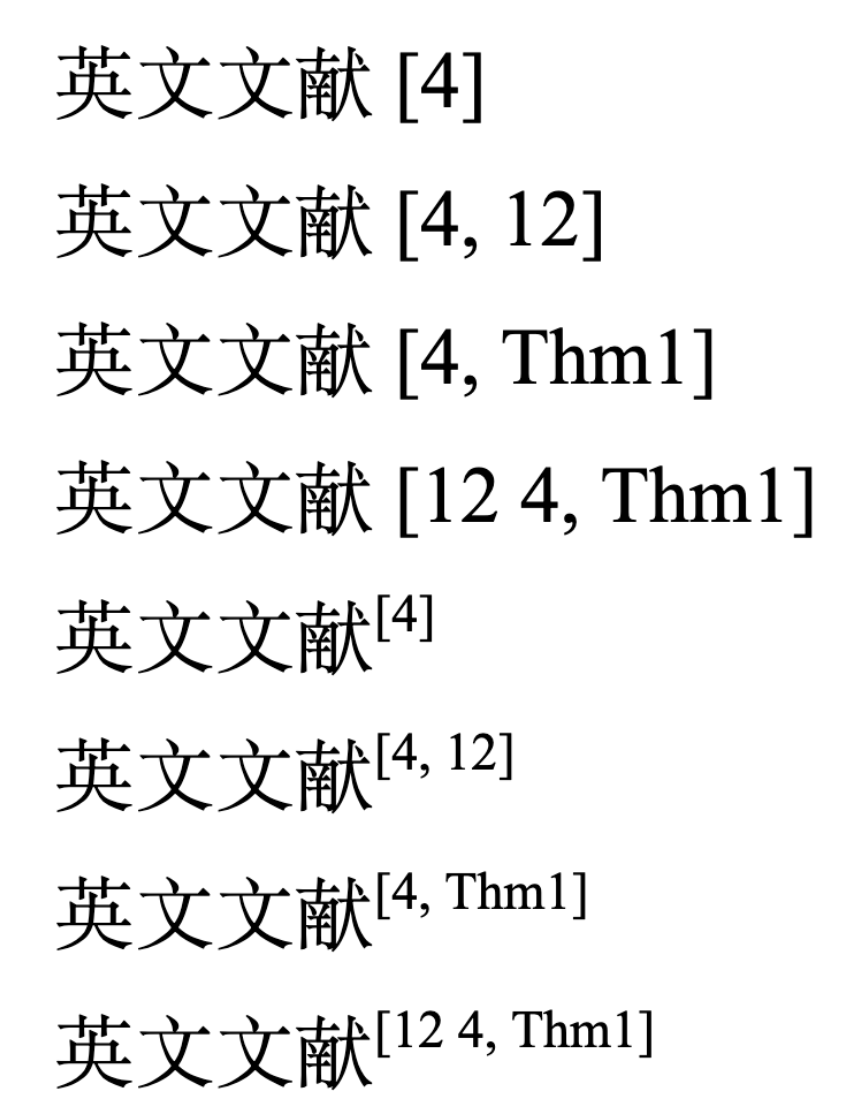
\includegraphics[width = 0.4\textwidth]{cite-parencite效果.png}
  \caption{\tn{cite} 和 \tn{parencite} 的效果}
  \label{figure:cite-parencite效果}
\end{figure}


\paragraph{定理类环境}


\begin{function}{axiom,counterexample,claim,corollary,conjecture,definition,example,lemma,property,proof,proposition,question,remark,theorem}
  \begin{ccnusyntax}[emph={[2]proof}]
    \begin{proof}(*\oarg{小标题}*)
      (*\meta{证明过程}*)
    \end{proof}
  \end{ccnusyntax}
  【本|硕|博】一系列预定义的数学环境。具体含义见表~\ref{tab:theorem}。
\end{function}

\begin{table}[ht]
  \caption{预定义的数学环境} \label{tab:theorem}
  \centering
  \small
  \begin{tblr}{
    width = \textwidth,
    columns = {c},
    hline{1,2,Z} = {solid}
  }
    \textbf{名称} &
      \env{axiom} & \env{counterexample} & \env{claim} & \env{corollary} & \env{conjecture} & \env{definition} & \env{example} \\
    \textbf{含义} &
      公理 & 反例 & 断言 & 推论 &
      猜想 & 定义 & 例 \\
  \end{tblr}

  \medskip

  \begin{tblr}{
    width = \textwidth,
    columns = {c},
    hline{1,2,Z} = {solid}
  }
    \textbf{名称} &
      \env{lemma} & \env{property} & \env{proof} & \env{proposition} & \env{question} & \env{remark} & \env{theorem} \\
    \textbf{含义} &
      引理 & 性质 & 证明 & 命题 &
      问题 & 注  & 定理 \\
  \end{tblr}
\end{table}

\begin{function}{\qedhere}
  【本|硕|博】证明环境(\env{proof})的最后会添加证毕符号“$\square$”。对于证明如果以公式结尾或其它某些情况时“$\square$”可能会出现在新的空白行的行尾,如果想要“$\square$”出现在“有内容的”行尾,可以在想要出现的地方使用 \tn{qedhere} 命令。
\end{function}

比如您可以在模板中测试下面代码查看效果:

\begin{latexexample}
  \begin{proof}
    \[
      x^2
    \]
  \end{proof}
  \begin{proof}
    \[
      x^2  \qedhere
    \]
  \end{proof}
\end{latexexample}


\begin{function}[added = 2022-06-04]{\ccnunewtheorem,\ccnunewtheorem*}
  \begin{ccnusyntax}[deletetexcs={\ccnunewtheorem,\ccnunewtheorem*},morekeywords={\ccnunewtheorem,\ccnunewtheorem*}]
    \ccnunewtheorem(*\oarg{计数器样式设置}\marg{环境中文名称}\marg{环境名}*)
    \ccnunewtheorem*(*\oarg{计数器样式设置}\marg{环境中文名称}\marg{环境名}*)
  \end{ccnusyntax}
  【本|硕|博】自定义定理类环境的命令。带星号的表示新定义的环境无计数器,类似于 \env{proof} 环境。
\end{function}

该命令的主要用法有下面四种:
\begin{latexexample}
  \ccnunewtheorem{测试}{test}
  \ccnunewtheorem*{测试试}{testt}
  \ccnunewtheorem[sibling = theorem]{测试试试}{testtt}
  \ccnunewtheorem[within = chapter]{测试试试试}{testttt}
\end{latexexample}

\begin{itemize}
  \item |\ccnunewtheorem{测试}{test}| 定义了一个 \env{test} 环境,label 名为 \env{测试}。环境自己用自己的计数器,并且跨 chapter 连续编号
  \item |\ccnunewtheorem*{测试试}{testt}| 定义了一个 \env{testt} 环境,label 名为 \env{测试试}。环境不编号。
  \item |\ccnunewtheorem[sibling = theorem]{测试试试}{testtt}| 定义了一个 \env{testtt} 环境,label 名为 \env{测试试试}。环境和 theorem 环境共用一个计数器。
  \item |\ccnunewtheorem[within = chapter]{测试试试试}{testttt}| 定义了一个 \env{testttt} 环境,label 名为 \env{测试试试试}。环境计数器的值和章节有关,形如 $x.y$,$x$ 表示章节的计数器的值,子计数器 $y$ 随新章节清零重新计数。
\end{itemize}

您可以看图~\ref{figure:ccnunewtheorem} 的效果来更好地理解四种用法的效果,

\begin{figure}[htbp]
  \centering
  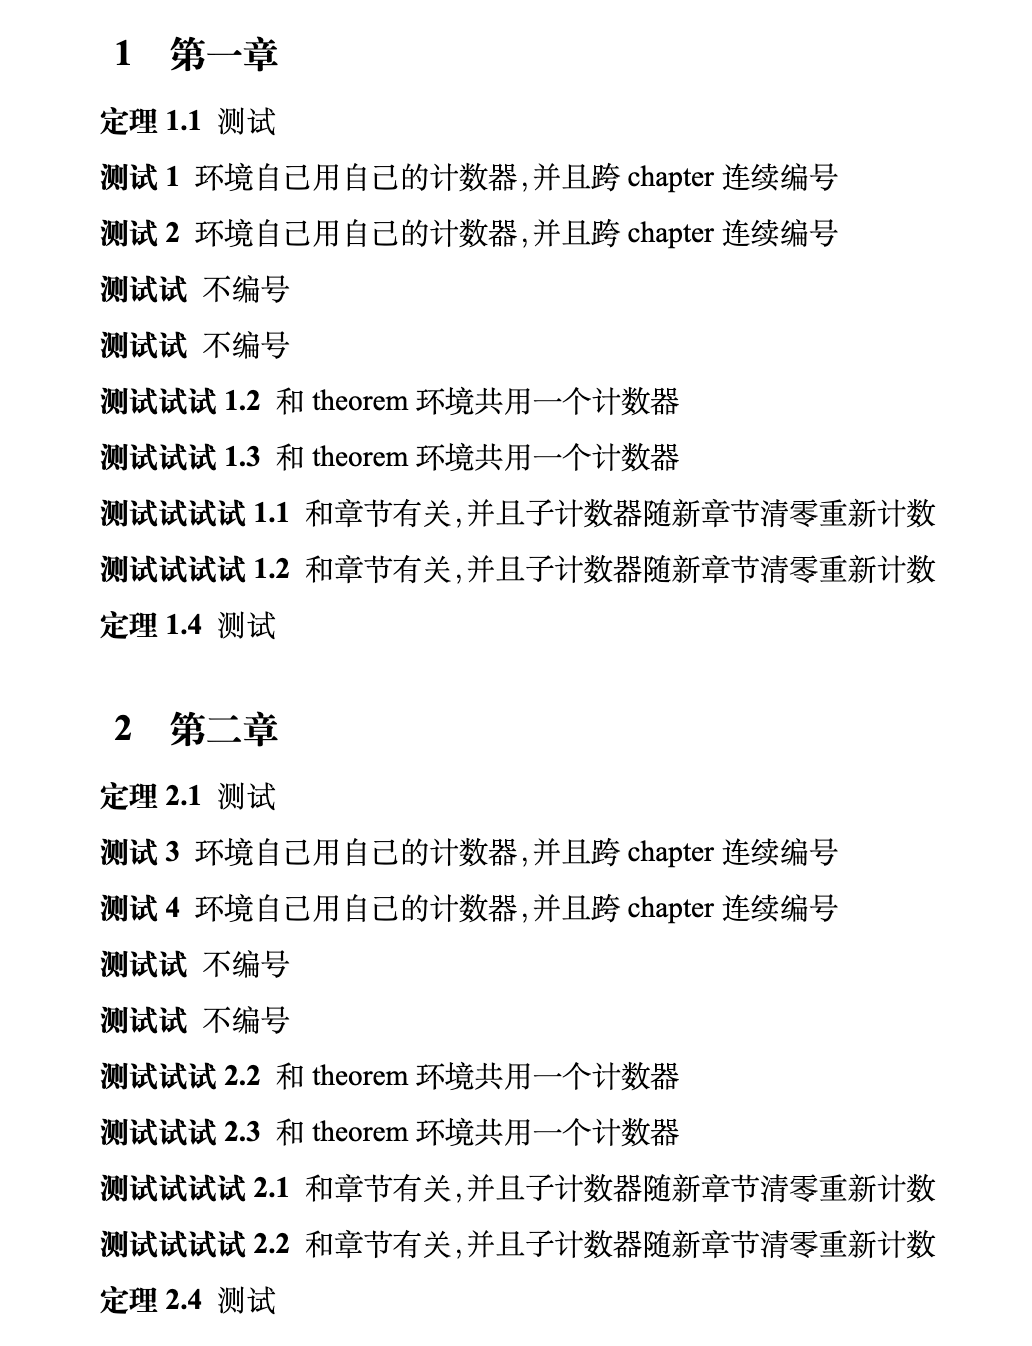
\includegraphics[width = 0.7\textwidth]{ccnunewtheorem.png}
  \caption{\tn{ccnunewtheorem} 示例}
  \label{figure:ccnunewtheorem}
\end{figure}



\subsubsection{豹尾}  \label{subsubsec:豹尾}

\begin{function}{\backmatter}
  【本|硕|博】声明后置部分开始。
\end{function}

后置部分包含参考文献、声明页等。

\begin{function}{\printbibliography}
  \begin{ccnusyntax}[morekeywords={\printbibliography}]
    \printbibliography(*\oarg{选项}*)
  \end{ccnusyntax}
  【本|硕|博】打印参考文献列表。该命令由 \pkg{biblatex} 宏包直接提供,可用选项请参阅其文档。一般来说,用户不需要做任何改动。
\end{function}

\begin{function}{\acknowledgements}
  【本|硕|博】开启致谢章节。

\begin{latexexample}
  % acknowledgements.tex
  \acknowledgements
  
  <致谢内容>
\end{latexexample}
\end{function}

\begin{function}[added = 2023-05-10]{\blind}
  【本|硕|博】在致谢或研究成果中需要去掉姓名、信息等的命令。

\begin{latexexample}
  我要感谢 CCNUthesis 的模板开发者 \blind{夏康玮}。
\end{latexexample}
如果开启盲审选项(见 \ref{subsec:模板选项} 节的 \opt{blind-version} 键值),即当文档类选项中(\tn{documentclass} 的可选参数中)是以下几种情况之一:
\begin{enumerate}
  \item \opt{blind-version}
  \item \kvopt{blind-version}{true}
  \item \kvopt{blind-version}{remove-partial-schoolname}
  \item \kvopt{blind-version}{remove-all-schoolname}
  \item \kvopt{blind-version}{blind-schoolname}
\end{enumerate}
则编译效果为
\begin{latexexample}
  我要感谢 CCNUthesis 的模板开发者***。
\end{latexexample}
否则就原封不动输出
\begin{latexexample}
  我要感谢 CCNUthesis 的模板开发者夏康玮。
\end{latexexample}
\end{function}

\begin{function}{signature}
  \begin{ccnusyntax}
    \begin{signature}
      <落款>
    \end{signature}
  \end{ccnusyntax}
  【本|硕|博】落款签名。整体右对齐,内部居中对齐。可用|\\|换行
\begin{latexexample}
  \begin{signature}
    夏康玮 \\
    2022年6月5日于珞珈山
  \end{signature}
\end{latexexample}
\end{function}


\begin{function}{\appendix}
  【本|硕|博】开启附录章节。
  
\begin{latexexample}
  % appendix.tex
  \appendix
  
  \chapter{<附录标题>}
  <附录内容>

  \chapter{<附录标题>}
  <附录内容>
\end{latexexample}

  附录和正文的章节层级相同,也是 \tn{chapter} 开始。需注意:\emph{硕博模板的附录在致谢前,本科模板的附录在致谢后。}

  根据 \parencite{研究生院研究生学位论文规范} 的要求“附录另起一页,“附录”两字居中,中间空两格,三号黑体加粗。如有多个附录,可用附录1、附录2区别并加以排序。” 模板已经做了自动化处理,即
  \begin{itemize}
    \item 如果 \file{appendix.tex} 中只有一个 \tn{chapter}\marg{内容} 的话,章节标题和目录中显示“附录 \meta{内容}”
    \item 如果 \file{appendix.tex} 中有两个及两个以上的 \tn{chapter}\marg{内容} 的话,章节标题和目录中显示“附录A \meta{内容}”、“附录B \meta{内容}”
  \end{itemize}
  但和一般的交叉引用不同,附录的此自动化处理,一般来说可能需要编译两次甚至三次,这个取决于用户在何时进行编译(比如编译之后又写了一个 \tn{chapter}\marg{内容} 的话,就需要三次编译才可以达到正确的章节标题和目录内容),但是三次(只要附录外的内容没问题,附录内没有报错)一定可以达到正确的编译效果。
\end{function}


\begin{function}{\publication}
  【博】开启“攻读学位期间取得的研究成果”章节。
\end{function}

\begin{function}{publications}
  \begin{ccnusyntax}[emph={[2]publications}]
    \begin{publications}
      \item (*\meta{研究成果1}*)
      \item (*\meta{研究成果2}*)
      ...
    \end{publications}
  \end{ccnusyntax}
  【博】研究成果列表环境。研究成果的格式等需要用户自行输入,无法像参考文献一样自动化,具体的字体字样等命令请自行查阅 \href{https://ctan.math.illinois.edu/info/lshort/chinese/lshort-zh-cn.pdf}{lshort-zh-cn}。
\end{function}

博士模板使用只需要取消 \file{main.tex} 中的
\begin{latexexample}
  % % !TeX root = ../main.tex
\publication


\begin{publications}
  \item test
  \item test
  \item test
  \item test
  \item test
  \item test
  \item test
  \item test
  \item test
  \item test
  \item test
  \item test
  \item test
  \item test
  \item test
  \item test
\end{publications}
\end{latexexample}
的代码注释,并且在 \file{publications.tex} 文件中输入相应内容然后编译即可。

\begin{function}{choices}
  \begin{ccnusyntax}[emph={[2]choices}]
    \begin{choices}(*\oarg{可选参数}*)
      \item (*\meta{选项1}*)
      \item (*\meta{选项2}*)
      ...
    \end{choices}
  \end{ccnusyntax}
  【本|硕|博】选项排版环境。对于有排版试卷、问卷等需求的用户,此环境能方便地帮您进行任意个选项的排版,并可以方便地调整选项 label 的样式。
\end{function}

用法和列表环境相同,使用 \tn{item} 分隔选项。label 的样式支持

\begin{itemize}
  \item arabic(阿拉伯数字)
  \item alph(小写英文)
  \item Alph(大写英文)
  \item roman(小写罗马数字)
  \item Roman(大写罗马数字)
  \item circlednumber(带圈数字)
\end{itemize}

如
\begin{latexexample}
  \begin{choices}[label = \arabic*)]
    \item 选项1
    \item 选项2
    \item 选项3
    \item 选项4
  \end{choices}
  
  \begin{choices}[label = (\alph*]
    \item 选项1
    \item 选项2
    \item 选项3
    \item 选项4
  \end{choices}
  
  \begin{choices}[label = \Alph*.]
    \item 选项1
    \item 选项2
    \item 选项3
    \item 选项4
  \end{choices}
  
  \begin{choices}[label = \roman*:]
    \item 选项1
    \item 选项2
    \item 选项3
    \item 选项4
  \end{choices}
  
  \begin{choices}[label = \Roman*-]
    \item 选项1
    \item 选项2
    \item 选项3
    \item 选项4
  \end{choices}
  
  \begin{choices}[label = \circlednumber*]
    \item 选项1
    \item 选项2
    \item 选项3
    \item 选项4
    \item 选项5
    \item 选项6
    \item 选项7
    \item 选项8
  \end{choices}
\end{latexexample}


还可以修改 \opt{columns} 键值来决定每行排多少个
\begin{latexexample}
  \begin{choices}[
    columns = 3,            % 手动控制每行多少个选项,否则自己根据宽度自动排版
    label   = (\arabic*)      % label 的样式,支持 arabic, alph, Alph, roman, Roman, circlednumber
  ]
    \item 选项1
    \item 选项2
    \item 选项3
    \item 选项4
    \item 选项5
    \item 选项6
  \end{choices}
\end{latexexample}

具体效果可见~\ref{figure:choices环境示例}。更多关于 \env{choices} 环境的精细调整可以查看 \url{https://gitee.com/zepinglee/exam-zh}。

\begin{figure}[htbp]
  \centering
  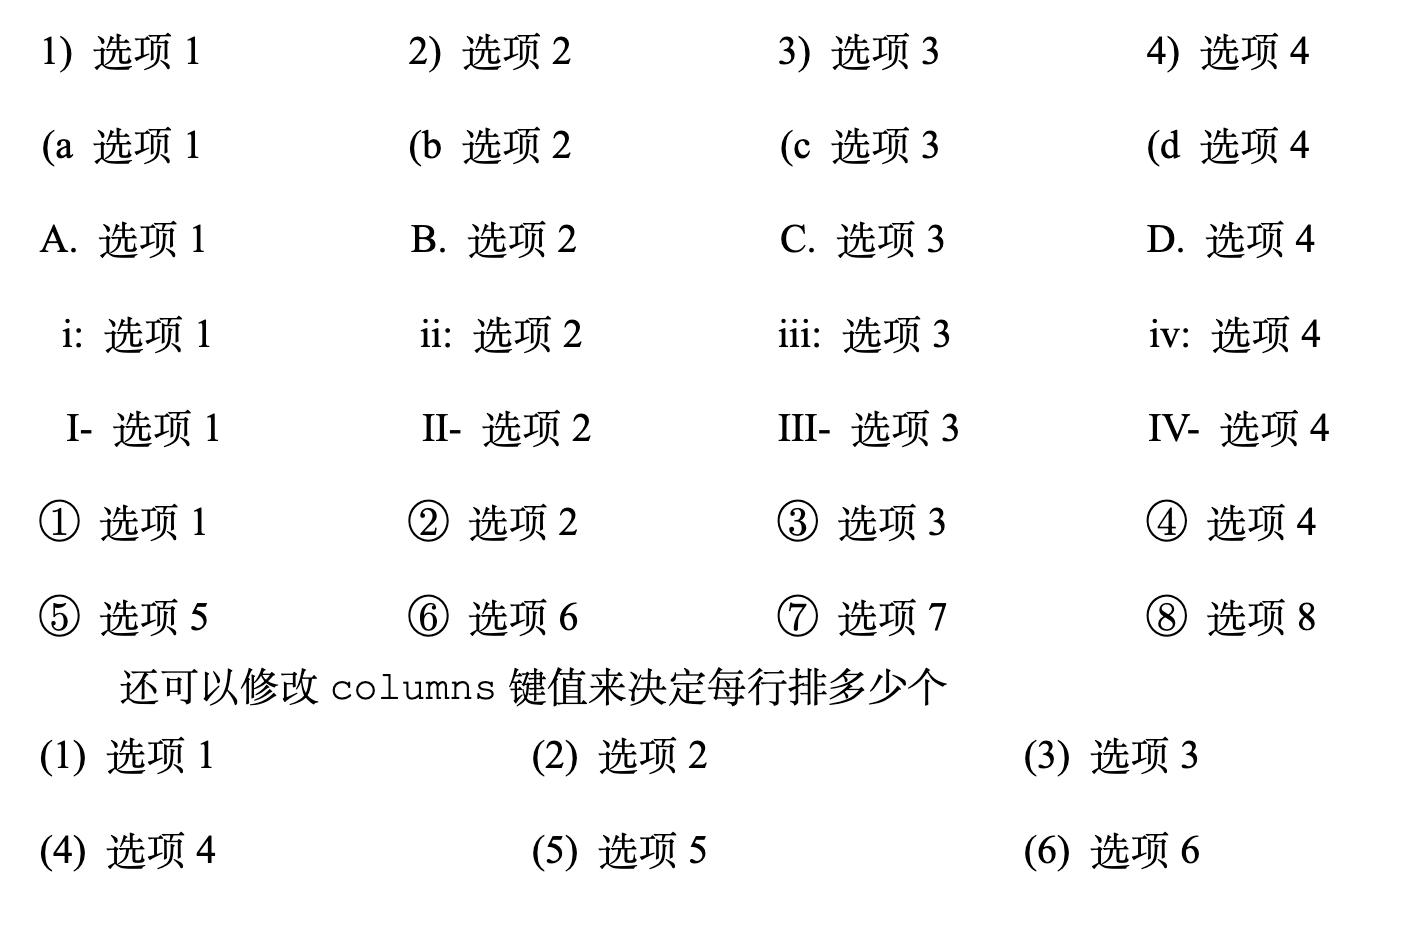
\includegraphics[width = 0.9\textwidth]{choices环境.png}
  \caption{\env{choices} 环境示例}
  \label{figure:choices环境示例}
\end{figure}